
\section{$\beta-$二羰基化合物}


\begin{center}
    \small
    \schemestart
    \chemfig{-[:30](=[:90]O)-[:-30]-[:30](=[:90]O)-[:-30]}
    \schemestop
\end{center}

有酸性,亲核性(容易与亲核试剂反应)

\subsection{丙二酸二乙酯}

丙二酸二乙酯的合成技巧是可以往中间那个 $\ce{C}$ 原子接烷基。如果用两个卤素原子放在中间,就可以接环等有趣的物质

\begin{figure}[H]
    \centering
    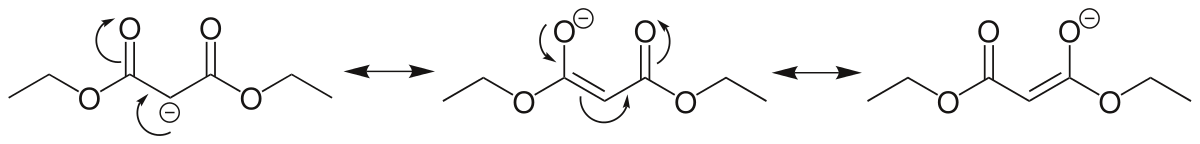
\includegraphics[width=0.7\textwidth]{img/1200px-Diethyl_malonate_resonance.svg.png}
\end{figure}

\begin{figure}[H]
    \centering
    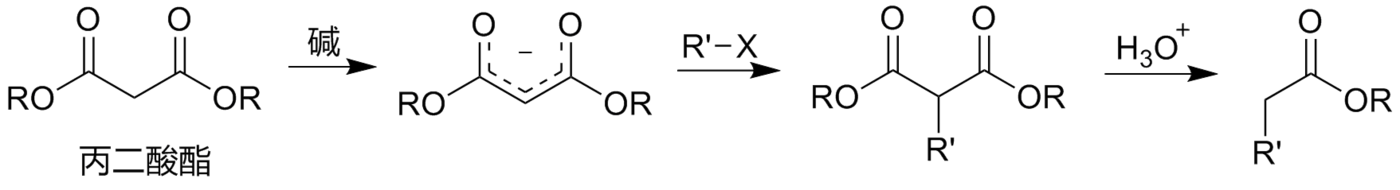
\includegraphics[width=0.8\textwidth]{img/1400px-Malonic_ester_synthesis_(zh).png}
\end{figure}

\subsection{反应机理}

\begin{figure}[H]
    \centering
    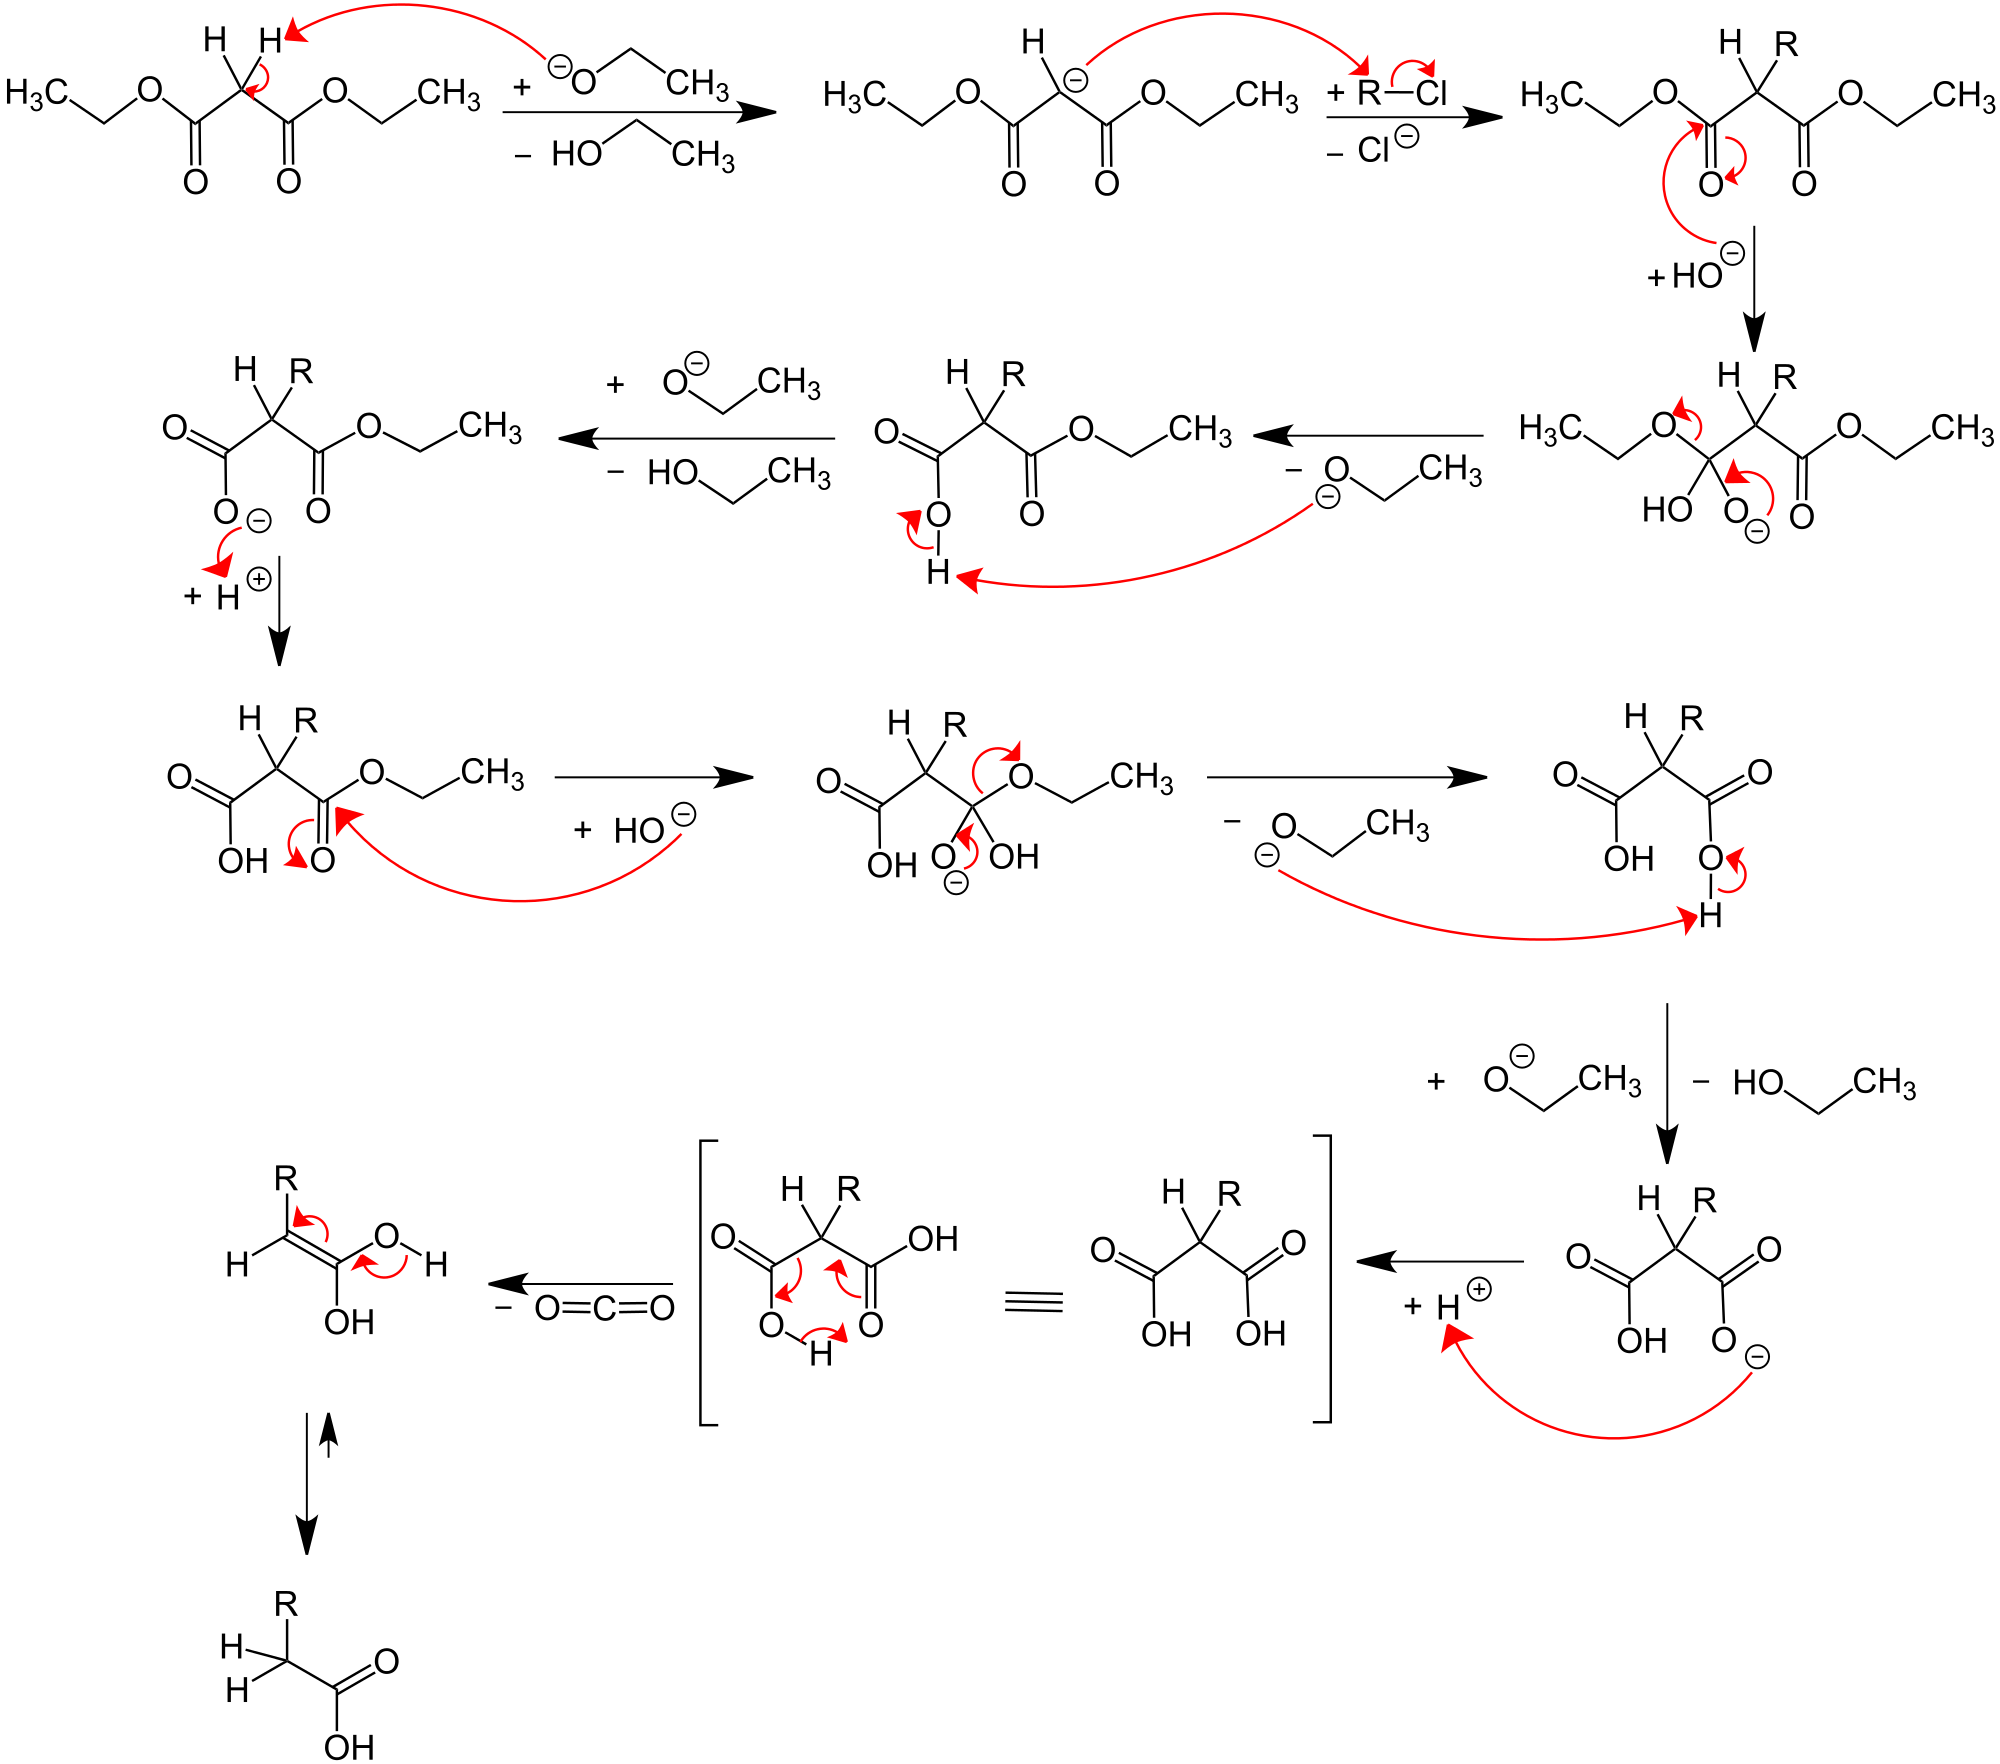
\includegraphics[width=0.9\textwidth]{img/2000px-Mechanismus_Malonestersynthese_V4.svg.png}
\end{figure}

\subsection{丙二酸二乙酯在合成上的作用}

\subsubsection{一元酸}

\begin{center}
    \scriptsize
    \schemestart
    $\ce{[CH(COO(C2H5)2)]Na+}$ \+ $\ce{CH3Cl}$ \arrow{->} $\ce{CH3CH(COOC2H5)2}$ \arrow{->} $\ce{CH3CH2COOH}$ 
    \schemestop
\end{center}


\subsubsection{环酸}

\begin{figure}[H]
    \centering
    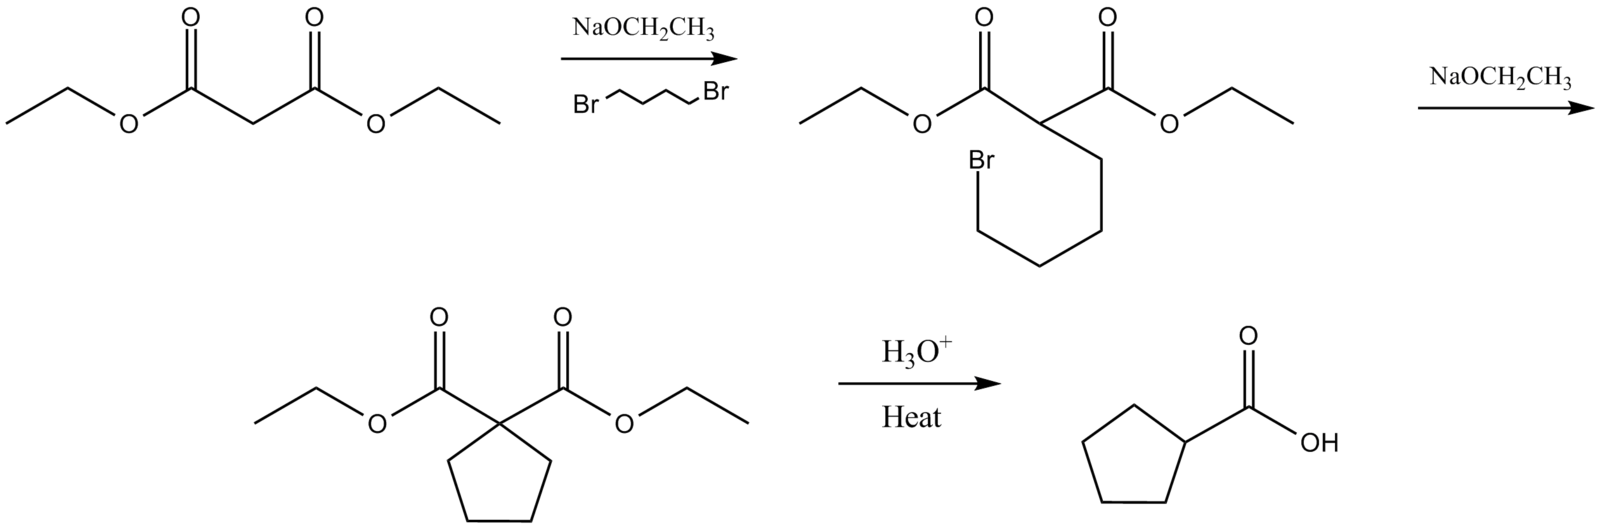
\includegraphics[width=0.9\textwidth]{img/1600px-Cycloalkylcarboxylic_acid_mechanism.png}
\end{figure}

\subsection{乙酰乙酸乙酯}

酸式分解、酮式分解。

酸式分解用的比较少,因为会伴随副反应。

酮式分解的条件:

\begin{center}
    \small
    \schemestart
    \arrow{->[$5\% \ce{NaOH}$ ][$\ce{H+}, \Delta$ ]}[,2.0]
    \schemestop
\end{center}

\begin{figure}[H]
    \centering
    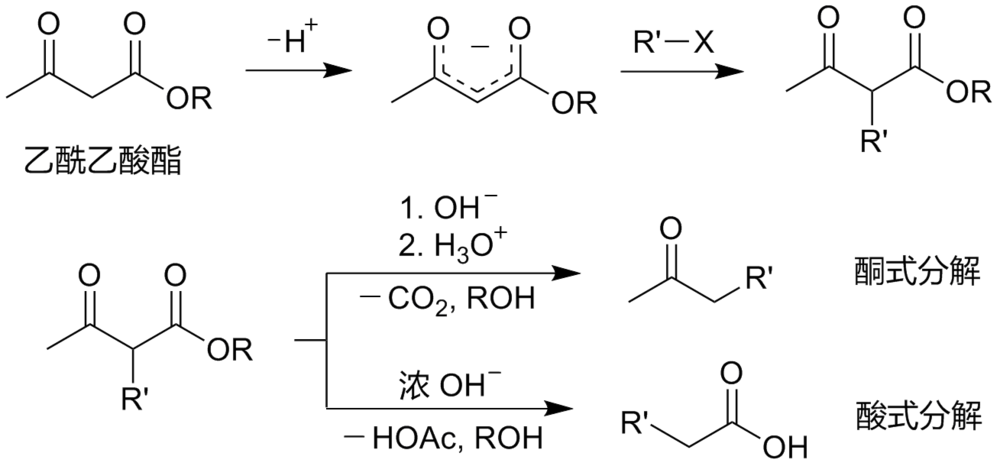
\includegraphics[width=0.9\textwidth]{img/AcetoaceticEsterSynthesis.png}
\end{figure}



\subsubsection{制备丁酮}

\begin{center}
    \small
    \schemestart
    \chemfig{-[:30](=[:90]O)-[:-30]CH_2CH_3}
    \schemestop
\end{center}


用 $\ce{CH3Cl}$ 直接和乙酰乙酸乙酯溶液混合,再酮式分解。


\subsubsection{制备二元甲基酮}

